\documentclass[tikz,border=3pt]{standalone}
\usepackage{lmodern}
\usepackage{xcolor}
\usetikzlibrary{arrows.meta}


\begin{document}
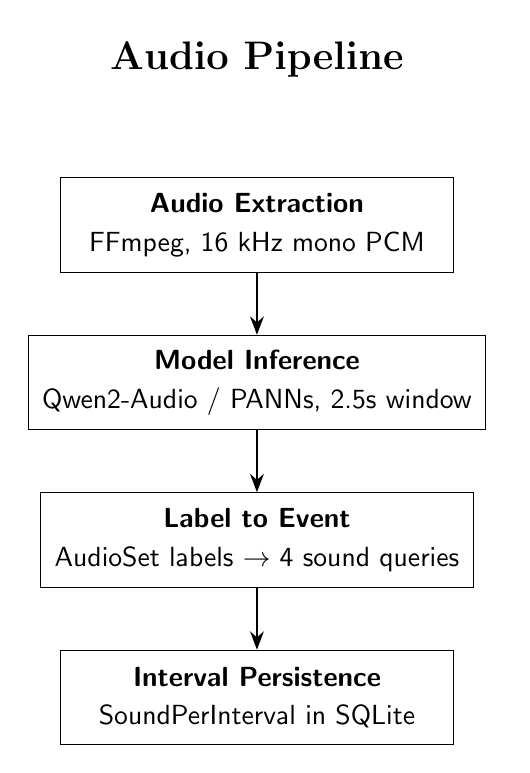
\begin{tikzpicture}[
  every node/.style={font=\sffamily},
  box/.style={draw=black, align=center, inner sep=5pt, minimum width=5cm, minimum height=1.2cm},
  arrow/.style={-Stealth, thick},
]

\draw[white] (-0.3,-0.5) rectangle (5.6,7.3);

\node[font=\Large\bfseries] at (2.5,6.9) {Audio Pipeline};

\node[box,fill=white] (s1) at (2.5,4.8) {
    \textbf{Audio Extraction}\\[2pt]
    FFmpeg, 16 kHz mono PCM
};

\node[box,fill=white] (s2) at (2.5,2.8) {
    \textbf{Model Inference}\\[2pt]
    Qwen2-Audio / PANNs, 2.5s window
};

\node[box,fill=white] (s3) at (2.5,0.8) {
    \textbf{Label to Event}\\[2pt]
    AudioSet labels $\to$ 4 sound queries
};

\node[box,fill=white] (s4) at (2.5,-1.2) {
    \textbf{Interval Persistence}\\[2pt]
    SoundPerInterval in SQLite
};

\draw[arrow] (s1.south) -- (s2.north);
\draw[arrow] (s2.south) -- (s3.north);
\draw[arrow] (s3.south) -- (s4.north);

\end{tikzpicture}
\end{document}
